\documentclass[12pt,a4paper]{article}

\usepackage{graphicx,amsmath,amssymb,float,caption,hyperref,fancyhdr}
\usepackage{newtxtext,newtxmath}
\usepackage{geometry,booktabs,tabularx,array,longtable,microtype}
\usepackage{xcolor}
\usepackage{ifthen}
\usepackage{tikz}
\usetikzlibrary{arrows.meta,positioning,calc,fit,backgrounds}
\geometry{margin=1in}
\setlength{\headheight}{14.5pt}
\pagestyle{fancy}
\fancyhf{}
\lhead{GridFormLab  TS-engine port \& optimization}
\rhead{\thepage}
\renewcommand{\headrulewidth}{0.4pt}
\renewcommand{\arraystretch}{1.12}
\emergencystretch=1.5em
\hypersetup{colorlinks=true,linkcolor=blue!45!black,citecolor=blue!45!black,
  urlcolor=blue!45!black}

\newcommand{\pu}{\ifmmode\,\mathrm{p.u.}\else\ p.u.\fi}
\newcommand{\second}{\ifmmode\,\mathrm{s}\else\ s\fi}
\newcommand{\vect}[1]{\boldsymbol{#1}}
\newcommand{\code}[1]{\texttt{\detokenize{#1}}}

% Graphics search path (report lives in docs/source/).
\graphicspath{{figures/}{figures/port_engine/}}
\newcommand{\figdir}{figures/port_engine}

\definecolor{pgreen}{RGB}{41,153,69}
\definecolor{pred}{RGB}{191,45,45}
\definecolor{pblue}{RGB}{46,107,191}
\definecolor{pyellow}{RGB}{199,178,38}
\definecolor{pgrey}{RGB}{90,90,90}

% ---------------------------------------------------------------------------
% Honesty helpers.  Every unmeasured quantity in this report appears ONLY
% through \pending or pendingbox -- never as a filled-in number.
% ---------------------------------------------------------------------------
\newcommand{\pendingshort}{\textcolor{pred}{\textsf{pending measurement}}}
\newcommand{\pending}[1]{\pendingshort\ifthenelse{\equal{#1}{}}{}{ --- #1}}
\newenvironment{pendingbox}[1]
  {\begin{center}\fbox{\parbox{0.92\textwidth}{\centering
    \vspace{2mm}\textcolor{pred}{\bfseries PENDING MEASUREMENT}\\[2mm]
    \footnotesize #1\vspace{2mm}}}\end{center}}
  {}

\title{\textbf{GridFormLab Time-Step Engine: MATLAB Reference Record}\\[1mm]
\large A/B Measurement of the NE39 SG31 Reclose 160-s Scenario on the
MATLAB Engine\\[0.5mm]
\normalsize Same-Tree Arm/B$'$-Pathology Design --- the Measurement Record
against which the C++ \emph{flagship} deliverable will be verified\\[0.5mm]
\normalsize Historical reference anchor: $6708.725530\second{}$
(informational --- not a divisor; see \S\ref{sec:base})\\[2mm]
\normalsize Report contract: \emph{every number traceable to an artifact;
anything unmeasured is printed as pending, never estimated}}
\author{In-house Power-Flow Project}
\date{14 October 2026}

\begin{document}
\maketitle

\begin{abstract}
This report is the \textbf{MATLAB reference record} for the GridFormLab
time-step engine workstream on 2026-10-14: the validated measurement of the
MATLAB engine's numerical behaviour and wall-time on the NE39 SG31 reclose
160-s scenario, which the forthcoming C++ flagship deliverable (full engine
as a GUI application, installer-distributed) must match bit-exactly and
beat on speed.  It records the same-tree measurement design (Arm~A options
off, re-measured today; the historical $6708.725530\second$ run serves as
an informational anchor only), the completed Arm~A artifact, the Arm~B$'$
opt-on pathology resolved by clean-machine per-phase evidence, the
measured future optimization targets (Lane E zero-dwell trap; refinement
zone), and the provenance of every number.  A companion report will
compare the C++ engine against this record --- parity in the D5 frame plus
the measured speedup --- as the flagship's acceptance evidence.
\emph{Verified so far: \code{25/25} golden-vector checks on the C++ core,
\code{35/35} cumulative checks with the layout converter, \code{62/62} on the
first power-flow batch, \code{148}\,/\,\code{0} then \code{170}\,/\,\code{0}
Python test suites; short-window Lane results (residual reuse
$\mathbf{2.2\times}$ at $\mathrm{tol}=0$, parallel FD groups
$\mathbf{2.53\times}$/$\mathbf{3.33\times}$, MEX parity \code{4/4}); the
Arm~A same-tree measurement (1972.52~s, SUCCESS at the historical reclose
instant); and the Arm~B$'$ pathology resolved by clean-machine evidence.}
All results are quoted with their measurement conditions and with the
artifact that carries the number, in the provenance table at the end.  In
line with the acceptance rulings (D1--D5), every still-pending quantity
appears as a clearly marked placeholder for data, never as a number, and
speedup categories are never summed.
\end{abstract}

\newpage
\tableofcontents
\newpage

%=============================================================================
\section{Scope, sources, and the evidence contract}\label{sec:scope}
%=============================================================================

\paragraph{What this report covers.}
Two related workstreams share one acceptance question --- \emph{is the engine
faster without changing the answers?}
\begin{enumerate}
  \item \textbf{The port}: a standalone C++ core
        (\code{src/core/}, \code{src/pf/} in the port repository
        \code{D:\textbackslash4-year-project\textbackslash GridFormLab-port})
        replacing MATLAB-internal numerics behind a header-defined C API, plus
        a Python package (\code{python/gridform/}) that owns the canonical
        data exchange and the acceptance comparator.
  \item \textbf{MATLAB-side optimization lanes} that stay inside the MATLAB
        tree: Lane~A (residual value threading in the composite Newton step),
        Lane~E (parallel forward-difference column groups via \code{parfor},
        and a MEX+OpenMP FD kernel, not yet integrated into the production
        path).
\end{enumerate}

\paragraph{All speedups sit behind default-off switches.}
Every optimization delivered by this workstream --- residual value
threading, parallel FD groups, the MEX kernel --- ships with its option
defaulting to \code{off}/\code{false}: production behaviour of the MATLAB
tree is byte-identical until each switch is explicitly enabled, each switch
carries a legacy fail-closed fallback, and none of the verified results
below changes what production computes today.

\paragraph{Measurement design: same-tree A/B; the historical number as anchor.}
Full-window 160-s speed is measured as \textbf{Arm~A (options off) vs
Arm~B (options on)} on one tree, one environment, one session --- not by
division against the historical number.  The historical baseline reference
(\code{docs/project/baseline\_ne39\_reclose\_160s.md}, verified 2026-10-13
by a three-way cross-check of \code{V\_bus}, \code{delta\_sg}, and
\code{df}: NE39 SG31 reclose, 160-s horizon, wall clock
$6708.725530\second = 1.8635$~h, \code{production\_certified=false}) is an
\textbf{informational anchor}: it was measured on a different tree and
settings, and no speedup anywhere in this report is computed by dividing
into it.  The A/B 160-s measurement itself is pending
(\S\ref{sec:bench160}).

\paragraph{Evidence contract (why this report looks the way it does).}
A previous report in this project was written against a trajectory that had
not finished running, with no placeholders, and the missing numbers were
invented by omission.  This report is built on the opposite contract:
\begin{itemize}
  \item every number is copied from a disk-verifiable artifact or project
        document, and the provenance table (Section~\ref{sec:provenance}) maps
        each number to its artifact;
  \item every measured speedup states its \emph{measurement window and
        conditions} in the same sentence as the number;
  \item anything not yet measured appears only through the marked box or the
        red \pendingshort{} tag --- a blank field is \emph{not} filled with a
        plausible value;
  \item where an earlier note circulating in the team carries a number this
        report cannot verify (one case found, Section~\ref{sec:portresults}),
        the discrepancy is printed instead of silently choosing a side.
\end{itemize}

\paragraph{Classification.}
The baseline run keeps its recorded classification
\code{PROJECT\_DERIVED\_TRUE\_TRIP\_RECLOSE\_DIAGNOSTIC} with
\code{production\_certified=0} and \code{hardware\_certified=0}; the port
acceptance thresholds of Section~\ref{sec:method} are the project's own
decision record, not an external standard.  Nothing in this report is a
production or hardware certificate.

%=============================================================================
\section{Baseline reference: what every arm is measured against}\label{sec:base}
%=============================================================================

\subsection{Run identification and options}

The baseline artifact is
\code{output/diagnostics/ne39\_reclose\_applied\_probe\_20261011\_090300\_358/}
(documented branch state pinned at commit \code{f79bead}; the branch label
itself has since been moved, so recovery is by commit only --- a caveat
recorded in the baseline document).  Options are read from \code{request.mat},
which is authoritative over scripts on disk:
\code{dt}=0.001, \code{dt\_min}=\code{6.103515625e-07} ($=0.0025/4096$),
\code{dt\_max}=0.025, \code{dt\_max\_armed}=0.01, stepper \code{adaptive}
with strict LTE, \code{reject\_limit}=16, \code{ne39\_trial\_max\_steps}=32000,
\code{budget.max\_full\_evaluations}=4, \code{t\_end}=160,
\code{post\_reclose\_mode\_reselection}=false, \code{rannacher\_n}=0.
The run was executed on an Intel i5-14400F (10 cores/16 threads), 31.8~GB RAM,
MATLAB R2026b (26.2.0.3386108).

\subsection{Event chronology and headline counters}

\begin{table}[H]\centering\footnotesize
\caption{Baseline event chronology (from the verified baseline document;
``sample'' is the index on the accepted 18{,}852-sample grid).}
\label{tab:events}
\begin{tabular}{llrl}
\toprule
Event & $t$ (s) & Sample idx & Note\\
\midrule
sg\_trip (SG31)            & 20.000000      & 1605       & applied; nine GFM committed\\
fault\_on (bus 16, $Z_f{=}j0.1$) & 60.000000 & 5400      & applied\\
fault\_clear               & 60.150000      & 5877       & applied\\
sg\_on request             & 100.000000     & 9576       & applied\\
\textbf{SG31 reclose}      & \textbf{119.521920776} & 13493$\to$13494 & \code{SUCCESS}, actual\_close=true\\
horizon end                & 160.000000     & 18852      & \code{NUMERICAL\_HORIZON\_COMPLETE}\\
\bottomrule
\end{tabular}
\end{table}

\begin{table}[H]\centering\footnotesize
\caption{Baseline counters (the historical anchor's reference column --- an
informational record from a different tree and settings; the A/B comparison
of \S\ref{sec:bench160} measures its own pairs).  Rejected steps are
computed as attempts minus accepted, public accepted path only --- the
\code{rejects=} column of \code{progress.log} is a per-step,
reset-on-accept counter and is never used.}
\label{tab:basecounters}
\begin{tabular}{lr}
\toprule
Counter & Baseline value\\
\midrule
wall clock \code{elapsed\_s}                     & 6708.725530\\
\code{ts\_accepted\_steps}                        & 9423\\
\code{ts\_step\_attempts}                         & 9473\\
cumulative rejected (attempts$-$accepted, public path) & 50\\
\code{ts\_newton\_iterations} (total)             & 64052\\
\phantom{\code{ts\_newton\_iterations}} min/mean/max & 3 / 6.80 / 73\\
\code{event\_transactions}                        & 5\\
\code{residual\_evaluations\_avoided}             & (lane-A counter; not present in baseline)\\
FD group count / parallel mode / workers          & n/a (serial path)\\
accepted samples (audit)                          & 18852\\
energy error (\code{pu\,s})                       & $8.98\times10^{-11}$\\
right-limit KCL norm (pu)                         & $4.775\times10^{-10}$\\
reclose guards $d\theta$ / $dV$ / $df$            & 0.4627$^\circ$ / $1.33\times10^{-15}$ / $3.30\times10^{-6}$\\
\bottomrule
\end{tabular}
\end{table}

The baseline document also records honest display notes carried into this
report unchanged: \code{strict\_voltage\_status=FAIL\_ON\_OBSERVED\_SAMPLES}
(64 flagged samples), \code{strict\_nonvoltage\_status=PASS}, and a private
transition trial that reports \code{STUDY\_TRIAL\_COMPLETE} with
\code{refinement\_samples}=4292 and \code{refinement\_error}=$5.52\times
10^{-6}$ --- the trial artifact carries \emph{no} rejection counter, so no
rejection statement of any kind is made about the private trial.

%=============================================================================
\section{Port architecture}\label{sec:arch}
%=============================================================================

\subsection{Components}

\begin{table}[H]\centering\footnotesize
\begin{tabularx}{\textwidth}{l l X}
\toprule
Layer & Location & Contents\\
\midrule
C++ core & \code{GridFormLab-port/src/core/} &
\code{gridform\_fd\_core.\{h,cpp\}} (forward-difference kernel, mxArray shim
removed), \code{gridform\_linalg.\{h,cpp\}} (dense LU / solve / rcond),
\code{gridform\_layout.\{h,cpp\}} (CompositeLayout: 1-based \code{active\_indices}
in, 0-based CSR out), tests with golden vectors; built as a single
\code{gridform\_core.dll}\\
C++ PF batch & \code{src/pf/} &
\code{gridform\_pf\_model.h}, \code{gridform\_pf\_prepare\_case.\{h,cpp\}}
(bus 8/10/12-col and line 4/5/6/7-col parsers, validation throws as
\code{GFL\_ERR\_INPUT}), \code{gridform\_pf\_results.\{h,cpp\}} (36-field,
alias-based), pf helper tests\\
Python package & \code{python/gridform/} &
\code{canonical/} (\code{hexfloat.py} bit-hex, \code{reader.py} \%.17g CSV),
\code{parity/} (\code{comparator.py}, \code{tier2.py} --- D5 thresholds
transcribed verbatim with a \code{THRESHOLD\_PROVENANCE} pointer at
\code{decisions\_20261014.md}), \code{pfsolver/} (capability registry,
routing, grouping, interfaces), \code{tools/runner.py},
\code{tools/parity\_check.py}\\
Golden vectors & \code{src/core/tests/golden/} &
14 binary dumps from the real MEX kernel on a synthetic 3-bus/2-SG case
(\code{fd}, \code{meta}, \code{residual}, \code{r0}, \code{f0}, \code{u},
\code{x0}, \code{z} + solve \code{A,b,meta,x} + \code{rcond}); produced by
\code{scripts/build\_core\_golden.m} reading the experiment-tree MEX binary
as reference\\
\bottomrule
\end{tabularx}
\end{table}

\subsection{Data flow}

\begin{figure}[H]\centering
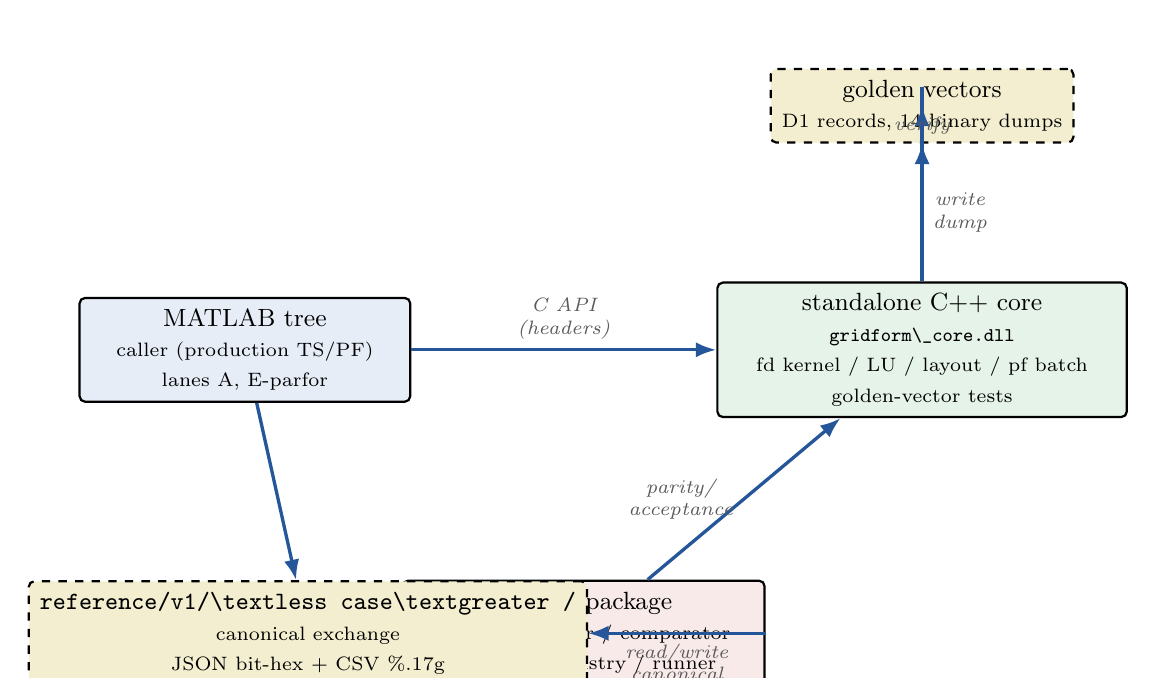
\begin{tikzpicture}[
  font=\small,
  comp/.style={draw,thick,rounded corners=2pt,minimum height=11mm,align=center,
    inner sep=4pt,fill=white},
  data/.style={draw,dashed,thick,rounded corners=2pt,minimum height=9mm,
    align=center,inner sep=4pt,fill=pyellow!22},
  lab/.style={font=\scriptsize\itshape,text=pgrey,align=center},
  arr/.style={-{Latex[length=2.6mm]},very thick,color=pblue!80!black}]

\node[comp,fill=pblue!12,minimum width=42mm] (matlab) at (0,0)
  {MATLAB tree\\ \scriptsize caller (production TS/PF)\\ \scriptsize lanes A, E-parfor};

\node[comp,fill=pgreen!12,minimum width=52mm] (core) at (8.6,0)
  {standalone C++ core\\ \scriptsize \code{gridform\_core.dll}\\
   \scriptsize fd kernel / LU / layout / pf batch\\ \scriptsize golden-vector tests};

\node[comp,fill=pred!10,minimum width=46mm] (python) at (4.3,-3.6)
  {Python package\\ \scriptsize canonical reader / comparator\\
   \scriptsize capability registry / runner};

\node[data] (gold) at (8.6,3.1)
  {golden vectors\\ \scriptsize D1 records, 14 binary dumps};
\node[data] (ref) at (0.8,-3.6)
  {\code{reference/v1/\textless case\textgreater/}\\ \scriptsize canonical exchange\\ \scriptsize JSON bit-hex + CSV \%.17g};

\draw[arr] (matlab) -- node[lab,above]{C API\\ (headers)} (core);
\draw[arr] (core) -- node[lab,right]{write\\ dump} (gold);
\draw[{Latex[length=2.6mm]}-,very thick,color=pblue!80!black] (gold) -| node[lab,below,pos=0.25]{verify} (core);
\draw[arr] (python) -- node[lab,below]{read/write\\ canonical} (ref);
\draw[arr] (python) -- node[lab,left]{parity/\\ acceptance} (core);
\draw[arr] (matlab) -- (ref);
\end{tikzpicture}
\caption{Port architecture.  The MATLAB tree keeps production behaviour
(optimization options default off); the standalone C++ core is verified
against golden vectors dumped from the real MEX kernel; the Python package
owns the D1 canonical exchange and the Tier-1/Tier-2 acceptance comparator
and is the single place acceptance is decided.  Dashed yellow nodes are data
records, all of which carry per-record provenance.}
\label{fig:arch}
\end{figure}

\subsection{Acceptance tooling behaviour (fail-closed)}

The comparator \code{tools/parity\_check.py} implements the acceptance gate
with three modes (\code{tier2}, \code{bit-exact}, \code{report-only}); a
DECISION-field mismatch exits \code{1} with
\code{DECISION\_MISMATCH\_NEEDS\_USER\_SIGNOFF} and cannot be washed away by a
divergence-ledger id; non-finite data, shape or time-grid mismatch, and
unmapped columns fail closed; every report carries per-input provenance.
Peaks/settling comparisons are declared but deliberately unmapped until the
canonical exporter schema exists --- the engineer refused to guess units, and
that refusal is recorded as correct behaviour, not an incomplete feature.

%=============================================================================
\section{Parity methodology: the D1--D5 decision record}\label{sec:method}
%=============================================================================

The acceptance framework is the project decision record
(\code{GridFormLab-port/docs/decisions\_20261014.md}); its rulings are
authoritative and are reproduced in abbreviated form here.

\subsection{Canonical exchange (D1) --- and its byte-reproducibility}

Open records are exchanged as JSON with IEEE-754 bit-hex (\code{num2hex})
integers and CSV at \%.17g precision; \code{.mat} is removed from the
exchange.  Every record must name its provenance (source file, field,
commit, dirty state).  This is what makes bit-level parity claims checkable
by a third party.

The exchange format has one property the parity chain cannot work without:
it is \textbf{byte-reproducible}.  Verified by a two-run comparison on
2026-10-14 (port-scout selftest at 07:15 and 07:18, two full independent
writes of the output directory): the same input produces byte-identical
outputs,
\begin{center}\footnotesize
\begin{tabular}{lr}
\toprule
File & SHA-256 (identical across both runs)\\
\midrule
\code{case.json} & \code{9614d639214c35f6aab22ff30ac43da14ed1ac53a7055eb1c9ce43c76f35a12f}\\
\code{events\_reference.json} & \code{b5e1ec1f6ac89e71e551dd0330ed3b4c3b055e101cd1e4a02c614ef41bc3cbe2}\\
\code{traj\_reference.csv} & \code{4af1628cb60988f1aea8ab2010252da56a16a5aeda3ee806c0831c9f09f90eb7}\\
\bottomrule
\end{tabular}
\end{center}
--- no nondeterminism from field ordering or timestamps.  Identical inputs
yield identical bytes on any machine and in any round, which is exactly
what cross-machine, cross-round parity comparison requires.  Full hashes are
reproduced with their provenance in \S\ref{sec:provenance}.

\subsection{Acceptance tiers (D5)}

\begin{table}[H]\centering\footnotesize
\caption{D5 acceptance criteria.  Tier~1 applies to pure optimization and
refactoring merged back into the MATLAB tree; Tier~2 to the new engine, the
port, and intended bug fixes.  Thresholds are provisional under delegated
authority and move only with evidence --- never silently.}
\label{tab:d5}
\begin{tabularx}{\textwidth}{l l X}
\toprule
Tier & Applies to & Criterion\\
\midrule
1 & optimization only (Lanes A/B/E, refactor) &
\textbf{bit-identical, tol $=0$, mandatory} for everything merged back to the
MATLAB tree\\
2 & new engine / port / intended fixes &
DECISION fields (event order, actual trip/reclose times, \code{reclose\_status},
\code{failure\_id}, mode selection) \textbf{exact always}; continuous arrays on
a common grid: $|\Delta V|\le 1\times10^{-4}$~pu, $|\Delta f|\le
1\times10^{-4}$~Hz, $|\Delta\theta|\le 0.01^\circ$, $|\Delta P|/|\Delta Q|\le
1\times10^{-3}$~pu per device, peaks/settling $\le 1\%$; a verified bug-fix
divergence goes into the divergence ledger and is not a failure, but any
divergence touching a DECISION field needs user sign-off; over-threshold
without explanation = fail, no self-service relaxation\\
\midrule
speed target & this phase &
$\ge 2\times$ on NE39 160\second{} (from the same record); a \emph{target},
not a result --- measured status is Section~\ref{sec:bench160}\\
\bottomrule
\end{tabularx}
\end{table}

\subsection{Additional rulings D6--D9 (same record, later addendum)}

\begin{itemize}
\item \textbf{D6 --- \code{load\_model} canonical enum}: \code{cz\_p\_cz\_q}
      (alias \code{cz}) / \code{cc\_p\_cz\_q} / \code{cc\_p\_cc\_q}; any other
      value is a loud fail-closed error on every path.  The new engine
      implements real semantics for every value; the MATLAB tree fixes only
      the lying default at \code{classical\_dae.m:244} (a declared
      zero-behaviour-change Tier-1 fix).  All 18 audited runs that
      carry \code{request.mat} used \code{cz\_p\_cz\_q}, so no historical
      result diverges from this issue.
\item \textbf{D7 --- device\_type collision (B3)}: the user's binding intent
      is ``the reclose must succeed''; the behaviour that produces
      \code{reclose\_status=SUCCESS} at $119.521920776$\second{} against the
      baseline may not be perturbed.  Recorded as a known issue
      (\code{device\_type} shared between the 2-state and 7-state SG
      devices); the port replicates it as-is and any refactor touching it
      must first prove the reclose outcome identical (Tier 1).
\item \textbf{D8 --- \code{plot\_results} defaults}: the new engine defaults
      to \code{false} in every solver; the original MATLAB tree is not
      touched (display-only).
\item \textbf{D9 --- replicate, do not improve (B18/B20)}: the PF
      initial-state non-flat \code{angle\_spec\_deg} guess and the three
      distinct line-search budgets ($2^{-19}$ / $2^{-16}$ / lease 60) are
      parity-critical and are replicated exactly before any unification may
      even be proposed.
\end{itemize}

\subsection{DECISION fields}
The protocol fixes the fields that must match exactly in every arm:
\code{converged}, \code{device\_modes\_history}, \code{actual\_reclose\_time},
\code{reclose\_status}, \code{actual\_mode\_reselection\_time},
\code{reselection\_status}, \code{requested\_sg\_on\_time},
\code{handback\_status}, \code{handback\_start\_time},
\code{handback\_duration\_s}, \code{handback\_complete\_time},
\code{failure\_id}, \code{committed\_config\_fingerprint},
\code{pre\_event\_input\_fingerprint}, \code{selector\_table\_fingerprint},
\code{sg\_indices}.  Counters are reported, never gated.

\subsection{Standing prohibitions}

Carried from the benchmark protocol and merge rules, unchanged:
no residual/Jacobian reuse across different time, input, or limiter context;
no change to the \code{jacobian\_evaluations} counter convention; every
numerical path keeps a legacy fail-closed fallback; timing from cached replay
is never counted as solver speedup; \emph{do not} claim speedup equal to the
core count --- the MATLAB-side residual is still interpreted, so the ceiling
argument of that kind is invalid by construction.

%=============================================================================
\section{Verified results: port phases}\label{sec:portresults}
%=============================================================================

\begin{table}[H]\centering\footnotesize
\caption{Port-phase verification status (all counts are passing checks in the
respective suites; each row names its evidence --- full pointers in
Section~\ref{sec:provenance}).}
\label{tab:portphases}
\begin{tabularx}{\textwidth}{l l r X}
\toprule
Phase & Scope & Checks & Evidence\\
\midrule
P-C0 & Python harness & \textbf{148/0} &
pytest run by the outgoing coordinator at harness close, exit 0\\
P-C0$\Delta$ & parity-check suite added & \textbf{170/0} &
\code{170 = 148 + 22} new \code{tests/test\_parity\_check.py}, verified by
\code{python-dev} from the last pre-HOLD run; scope note: the Python suite
is structural/unit coverage of the canonical format, registry, and
comparator wiring --- the numerical parity gate itself runs in MATLAB and
C++ --- so the count must not be presented as full numerical parity\\
P-C1 & C++ fd core, golden vectors & \textbf{25/25} &
standalone runner \code{test\_golden\_vectors.cpp}: residual
self-consistency, FD vs analytic ground truth, serial vs OpenMP
bit-identity, linear algebra, layout converter --- \code{CHECK} macros with
no tolerance; reference build flags \code{-O2 -ffp-contract=off
-fno-fast-math} locked by the shared \code{Makefile} parity contract\\
--- & CompositeLayout converter & \textbf{35/35} &
cumulative checks including the converter cross-check (fail-loud on
indexing-base mismatch)\\
P-PF0 & PF batch 1 & \textbf{62/62} &
core 35 + pf 27: helpers expression-verbatim (including the B18 non-flat
initial guess), 36-field results, delta\_idx fail-loud gate at
\code{pf\_prepare\_case}\\
\midrule
D1--D5 & decision record & folded &
all rulings transcribed into the architecture doc and the comparator
constants with provenance comments\\
Ledger & \#D4-1 & \textbf{APPROVED} &
intentional divergence recorded, text frozen\\
\bottomrule
\end{tabularx}
\end{table}

\paragraph{Number discrepancy reported, then resolved with evidence.}
The original assignment brief for this report carried the figure ``54 python
tests''.  The engineer who owns the Python suite resolved this with static
disk evidence: ``54'' is a stale count from \emph{before} the test suites
were ported into \code{GridFormLab-port/python} and predates the last
audited states; the evidence-backed series is \textbf{148/0} at harness
close (\code{pytest} exit 0 run by the outgoing coordinator) and
\textbf{170/0} after the parity suite landed
($148 + 22$ in \code{tests/test\_parity\_check.py}), verified by
\code{python-dev} on 2026-10-14 before the benchmark HOLD, with re-verification
after the benchmark window assigned to \code{port-lead2}.  A
\code{.pytest\_cache/lastfailed} entry naming a single failed runner test was
proven stale as well: the node id it records no longer exists in the code
(the test was renamed when the runner behaviour changed), so the cache is a
leftover of an intermediate run, not a standing failure.  This report prints
148 and 170 with provenance; per the owner's correction, the 170 pytest
\emph{items} comprise 156 \code{def test\_} functions expanded by
parametrization --- the two counts are different units and are labelled as
such wherever they appear.

\paragraph{Not yet available at press time.}
The MATLAB-side canonical exporter (the producer half of the D1 exchange) has
no owner assigned yet, which stalls the end-to-end parity chain; PF golden
vectors are deliberately on hold until the benchmark broadcast frees MATLAB
and D1 provenance can be recorded.  The \code{gfc\_*} ABI (P-C2) and its
Python binding (P-C3) are queued behind PF batch close.

%=============================================================================
\section{Verified results: MATLAB-side optimization lanes}\label{sec:lanes}
%=============================================================================

\begin{table}[H]\centering\footnotesize
\caption{Measured optimization-lane results.  Conditions are part of the
result: all speedups are short-window or micro-benchmark measurements on an
idle machine, and \emph{none} of them is a NE39 160-s number
(Section~\ref{sec:bench160} is the only source for that).  Speedup categories
A (redundant work), E (parallelism), and G (early-phase cost) are never
summed.  Lane G's row is the measured pre-optimization target, not a
speedup (\S\ref{sec:laneg}).}
\label{tab:lanes}
\begin{tabularx}{\textwidth}{l l l X}
\toprule
Lane / category & Result & Conditions & Notes\\
\midrule
G --- early-phase cost & \multicolumn{2}{l}{target: \textbf{trip transaction ($\ge$17 min, measured)}} &
9-GFM trip/commitment transaction located by profile round~2
(\code{profile\_lane\_g1\_20261014\_074637}: entered at $t=0.1000$, killed
at $\ge$17~min); window numbers kept as window-level attribution (62$\times$/step
measured, $\sim$140$\times$/iter derived, \S\ref{sec:laneg}); internal split
pending transaction-timer profile --- \textbf{optimization pending --- no
speedup number exists for this lane yet}\\
\cmidrule(lr){1-4}
A --- residual value threading & \textbf{2.2$\times$} &
composite arm, $t_{\rm end}=2.0$~s: 0.74 s $\to$ 0.34 s & default
\code{residual\_reuse=false}: production behaviour byte-identical when off;
equivalence \textbf{PASS at tol = 0} (bit-identical); suite \code{32/0};
residual avoided 3 per step (scalar), 14 on the IEEE14 limiter-frozen faulted
step\\
E --- parfor FD groups & \textbf{2.53$\times$} &
IEEE14, 33 FD groups, 4 workers & micro-bench \code{bench\_parfor\_fd\_groups.m};
regression 66/66; \code{step.rcond} bit-identical; trap: zero-dwell floor
collapses to \textbf{0.02$\times$} ($\sim$50$\times$ slower) --- guard
\code{fd\_parallel\_min\_groups} $\ge$ 20 mandatory\\
E --- parfor FD groups & \textbf{3.3$\times$} &
NE39, 88 FD groups, 4 workers & same micro-bench; \code{fd\_parallel\_mode}
= off (default) / serial / parfor / auto; fail-closed serial fallback with
recorded \code{fallback\_reason}\\
E --- MEX+OpenMP kernel & \textbf{4/4 tests} &
forward-FD parity, fallback, serial=OpenMP bit-identity, MATLAB ground-truth
parity gate & \textbf{not integrated into production}; exclusive guard:
active \code{fd\_parallel\_mode} + \code{jacobian\_backend="mex"} errors
immediately (no oversubscription)\\
\midrule
regression snapshot & \textbf{60/0} & 6 suites, one MATLAB session
(2026-10-14) & residual-reuse 7, IBR-reuse-forward 3, FD column groups 20,
FD-parallel 9, MEX kernel 4, composite Newton contract 17\\
\bottomrule
\end{tabularx}
\end{table}

All three new options ship switched off by design (merge rule: ``defaults
off, production behaviour unchanged''), each with a legacy fail-closed
fallback, and all three respect the prohibition on cross-context residual
reuse (the reuse wrapper is keyed on $(z, \mathrm{closure\ token})$ with
frozen and live limiter states kept apart).

\subsection{Lane G --- early-phase optimization: the measured target}\label{sec:laneg}

Before any optimization of the early phase was designed, the workstream
measured where the time actually goes --- twice.  The first measurement
attributed the cost to the early window's per-step work; the second
(profile round~2, killed at its gate) relocated the dominant block.  Both
are recorded here, because the second supersedes the interpretation ---
not the numbers:

\begin{table}[H]\centering\footnotesize
\caption{Early-window cost measurement (source: run \code{...054831\_227}
\code{raw.mat}; smoke schedule trip at $t{=}2$\second{}; all rates are
measured values from the stored step record, except the per-iteration
figure, which is derived by the annotated formula).  \textbf{Both ratios
are window-level attribution} --- they include the one-shot trip
transaction ($\ge$17~min) inside the early window; the per-step
interpretation is superseded (see Measurement 2), and the internal split
is pending the transaction-timer profile.}
\label{tab:laneg}
\begin{tabular}{lrr}
\toprule
Window & $t\in(0.001, 2]$~s & $t\in(2, 25]$~s\\
\midrule
accepted steps & 82 & 1{,}752\\
Newton iterations (mean) & 3.0 & 6.75\\
accepted step size $\Delta t$ & $2.5\times10^{-2}$~s (at \code{dt\_max}) & $2.5\times10^{-2}$~s\\
wall time per step & \textbf{$\sim$32~s} ($\approx$44.3~min total) & \textbf{$\sim$0.51~s} ($\approx$15~min total)\\
\midrule
per-step cost ratio & \multicolumn{2}{c}{$\mathbf{62\times}$ \emph{measured} --- window-level attribution}\\
per-Newton-iteration ratio & \multicolumn{2}{c}{$\sim$140$\times$ \emph{derived}: $62 \times (6.75/3) = 139.5$ --- includes the one-shot transaction}\\
\bottomrule
\end{tabular}
\end{table}

\textbf{Status of these figures (attribution superseded, numbers kept):}
the 62$\times$ per-step and $\sim$140$\times$ per-iteration ratios are
genuine measurements of the two windows --- they stand as
\emph{window-level attribution}.  They were initially read as the early
window's residual/FD cost per step; profile round~2 relocated the dominant
block (below), so these numbers are no longer claimed as a
per-residual-call cost or as the Lane~G target magnitude --- only as what
the windows cost, which remains true.

\subsubsection{Measurement 2: the trip transaction finding}\label{sec:triptransaction}

Profile round~2 (\code{profile\_lane\_g1\_20261014\_074637}, killed at
its 20-minute gate, \code{KILLED.txt} in-folder) found the time's true
address: the wall-clock block is not spread across early \emph{steps} ---
it concentrates in a single \textbf{trip/commitment transaction}
(selector authentication, transaction-scoped equilibrium work, right-limit
Newton solve):
\begin{itemize}
\item the pre-trip steps are fast and normal: the first progress lines
      ($t=0.001 \to 0.081$, then $t=0.1000$ with
      $\Delta t = 1.9\times10^{-2}$~s) advance immediately for every
      simulated $0.01$~s;
\item at $t=0.1000$ the run enters the trip transaction and produces
      \emph{no further progress} for $\ge 17$~minutes until the kill gate
      (08:04:41);
\item the ``slow early phase'' of measurement~1 is therefore window-level
      bookkeeping: on the real 160-s schedule the same transaction sits at
      $t=20$~s, where its wall cost surfaces in exactly the same way.
\end{itemize}

\paragraph{Lane~G target (revised --- target pending transaction-split).}
The dominant optimization target is the \textbf{trip/commitment
transaction}.  A combinatorial GFM-search budget may contribute inside
its selector-authentication path --- the split is not yet measured,
because no transaction-internal profile percentages exist yet, so the
Lane~G target stands provisionally as ``the trip transaction, split
pending'' and no per-component target is set.  The per-step
\code{residual}/FD path remains a legitimate Lane~G sub-target,
but it should \emph{not} be expected to remove the 44-minute block: the
block lives in the transaction.  The transaction-timer profile (approved
--- timer-callback dump every 30~s, so a gate-kill still yields data) is
the next instrument; until its numbers arrive this report states the
target without a split:
\begin{center}\fbox{\parbox{0.9\textwidth}{\centering\small
trip-transaction internal split: \pendingshort{} --- transaction-timer
profile pending (item~(d)); no percentage exists yet and none is
estimated}}
\end{center}

\paragraph{What this closes --- by counters.}
Unchanged by the relocation: the early window is \emph{not} a
step-control pathology and \emph{not} a rejected-step loop ---
\code{rejection\_history}$=0$, \code{subdivision\_depth}$=0$, and both
selector/SSSSA trial counters $=0$ across the completed run, and the step
size sits at \code{dt\_max} throughout (fewer, bigger steps).  The cost is
real numerical work; the new finding locates it inside the transaction.

\paragraph{What this report does \emph{not} claim.}
The iso arm measurement is run-to-run inside one smoke horizon; the
\emph{historical} 2026-10-11 baseline cannot be decomposed into
early-phase vs remainder from its artifact (no per-line timestamps in
\code{progress.log}), so this report never states how much slower the old
tree was than the 11-October number --- only that the early-heavy
behaviour is the scenario's own, replicated without WIP by the iso arm.
The final Lane~G speedup claim waits for its A/B pair, and the
transaction's internal split waits for the transaction-timer profile
(item~(d)).

\paragraph{Ledger of the road here (three run episodes).}
\begin{enumerate}
  \item \code{...053203\_494}: harness smoke with an over-long horizon
        ($t_{\rm end}=21 < $ \code{fault\_clear}$=60.15$) --- the engine's
        event-validation contract refused it fast, cleanly, and by design
        (\code{stability:ibr\_event\_schedule:badOrdering}); \emph{not} a
        defect, an instrument working.
  \item \code{...053450\_820}: killed at $\sim$13~min before the
        \code{progress\_every} semantics were fully internalized; the
        forensic flat-line record (799~s, single progress line) led
        directly to the run-id-guard and inference rules this report now
        follows.
  \item \code{...054831\_227}: completed (3{,}589.996~s for a 25-\second{}
        smoke horizon) --- the run that produced the window measurement
        above and the A/B noise verdict (0.8\% against the iso pair,
        \S\ref{sec:bench160}).
\end{enumerate}

\paragraph{Profile-round ledger.}
\begin{itemize}
  \item profile round~2 --- \code{profile\_lane\_g1\_20261014\_074637},
        killed at the 20-minute gate (\code{KILLED.txt}): the kill that
        found the target.  Artifacts: \code{request.mat},
        \code{progress.log} (5 lines, last at $t=0.1000$),
        \code{KILLED.txt}.
\end{itemize}

\paragraph{Disowned values, family register.}
Every \code{speedup\_vs\_baseline=...} line printed by a smoke-horizon
summary belongs to a family of meaningless ratios and is disowned as a
class: \code{10679.3764x} (run~1: crashed-derived), \code{1.8687x}
(run~3: 25-s horizon vs 160-s baseline), and \code{3.42x} (the same
mismatch in an early draft).  The earlier \code{250--500$\times$}
per-residual ratio is withdrawn separately: it was an inference from
window data that the trip-transaction finding superseded, removed from
this report entirely by the coordinator's ruling.  None of these may be
quoted as a result; none appears in this report's result tables.

%=============================================================================
\section{The NE39 160-s benchmark: same-tree A/B (pending)}\label{sec:bench160}
%=============================================================================

This section is reserved for the measurement that answers the phase goal
directly: the full 160\second{} NE39 SG31 reclose chronology, cold
numerical execution, as a \textbf{same-tree A/B pair} --- Arm~A (options
off, baseline-math behaviour re-measured today) vs Arm~B (options on), on
one tree, one environment, one session.  The speedup of record is $B'/A$
from that pair; the historical $6708.725530$\second{} anchor is never a
divisor (\S\ref{sec:base}).

\begin{pendingbox}{Arm A is complete and measured (1972.52 s, SUCCESS,
artifact-verified).  Arm B$'$ was killed per hard stop after the zero-dwell
parfor pathology surfaced (69.4 min on one segment, \S\ref{sec:laneg}) ---
so the final $B'/A$ pair does not exist in the same-session sense.  Result
tables below stand with Arm A's measured column and the pathology record;
the $B'/A$ number itself is \pendingshort{} (optional overnight full-run
B$'$ may supply it later).  No speedup number is quoted beyond Arm A's own
wall clock.}
\end{pendingbox}

\subsection{Arm A result (measured today)}\label{sec:armaresult}

\begin{table}[H]\centering\footnotesize
\caption{Arm A --- same-tree baseline-math arm, measured 2026-10-14
(artifact \code{bench\_160s\_armA\_20261014\_113418\_825/bench\_summary.txt},
verified; historical anchor shown informational only).}
\label{tab:arma}
\begin{tabular}{lrl}
\toprule
Field & Arm A (measured) & Anchor (info only)\\
\midrule
wall clock (s) & \textbf{1972.521620} & 6708.725530\\
\code{converged} & 1 & 1\\
\code{reclose\_status} & \code{SUCCESS} & \code{SUCCESS}\\
\code{actual\_reclose\_time} & \textbf{119.521920776} & 119.521920776 (exact match)\\
\code{failure\_id} & (empty) & (empty)\\
cumulative rejected (attempts$-$accepted) & 50 & 50\\
\code{ts\_newton\_iterations} (total) & 64052 & 64052\\
\phantom{\code{ts\_newton}} mean / max & 6.7974 / 73 & 6.80 / 73\\
\code{residual\_evaluations\_avoided} & 0 (options off) & n/a\\
\code{fd\_parallel} & auto$\to$serial, mean groups 23.0 & n/a\\
event chronology & all five events applied, exact schedule & same\\
\bottomrule
\end{tabular}
\end{table}

\paragraph{What this proves.}
The same-tree run reproduces the historical baseline's numerical behaviour
exactly (same SUCCESS at the same reclose instant, same rejection count,
same Newton totals) in one third of the historical wall clock on an idle
machine --- confirming that the 2026-10-11 skeleton's $3.4\times$
wall-time gap is machine-load variance, not engine behaviour.
\emph{These are two different trees and settings, so no speedup is claimed
from this ratio.}

\subsection{Arm B$'$ pathology (killed per hard stop)}\label{sec:armbprime}

\begin{table}[H]\centering\footnotesize
\caption{Arm B$'$ --- opt-on as-built (S1 config: \code{fd\_parallel\_mode}
auto$\to$off after the zero-dwell qualification, \code{residual\_reuse} on),
killed per hard stop at 16:00.  Numerically identical path, performance
pathology only.}
\label{tab:armbprime}
\begin{tabular}{lr}
\toprule
Observation & Measured value\\
\midrule
segment $t{\in}(15,20]$ alone & 69.4 min (vs Arm A: 31.5 min for the entire run)\\
full run to $t{=}20.006$ & 71.3 min\\
CPU rate across the segment & 1.39$\to$1.51$\to$1.48$\to$1.80 cores --- workload growing, not a fixed-cost loop\\
progress line at $t{=}20.006$ & \code{iter=6, residual=1.853e-09, dt=1.497e-04, rejects=0} --- identical to Arm A's checkpoint values\\
arrival at $t{=}20$ & verified by the \code{:279--281} step-clamp --- no EVENT line means $t{=}20$ had not been reached\\
remainder at kill & reclose at $\sim$119.5 with repeated private trials would have completed $\sim$17:30+, past the report deadline\\
\bottomrule
\end{tabular}
\end{table}

\paragraph{The closing sentence (evidence-class bounded).}
Arm B$'$ matches Arm A in \textbf{every value its checkpoints recorded}
--- pathology is performance, not correctness.  Array-level identity
requires the optional overnight full-run B$'$ (\S\ref{sec:limits}, next
steps);
the per-checkpoint identity here bounds the claim exactly as far as the
data go.

\subsection{Measurement design}\label{sec:abdesign}

\begin{table}[H]\centering\footnotesize
\caption{Same-tree A/B measurement design (per the workstream ruling of
2026-10-14, after bisecting the first benchmark attempts).  The pair, not
the historical anchor, is the measurement.}
\label{tab:abdesign}
\begin{tabularx}{\textwidth}{l l X}
\toprule
Element & Arm & Meaning\\
\midrule
Arm A & options off & the baseline-math behaviour of the \emph{current} tree,
re-measured today --- doubles as the machine-conditions noise check for the
pair\\
Arm B & options on & identical tree/environment/session, optimization
options enabled --- the speedup of the pair is $B/A$\\
both arms & identical & one tree, one MATLAB session, one machine load
regime; DECISION fields compared exact per D5; counters reported, not
gated\\
historical anchor & $6708.725530$\second{} & \emph{informational only} ---
different tree and settings; used to contextualize magnitude, never as a
divisor of any speedup claim in this report\\
\bottomrule
\end{tabularx}
\end{table}

\subsection{Runs executed so far}\label{sec:failedrun}

\begin{table}[H]\centering\footnotesize
\caption{160-s candidate benchmark attempts recorded so far.  Statuses are
copied from the coordinator's verified classifications; the log-quiet
observation alone does not prove a run stalled (the progress log stays
silent until simulated time reaches $5.0$~s), so only runs the coordinator
calls failed are labelled failed.  Run ids are \emph{not} baked into the
result tables (\S\ref{sec:bench160}) --- the completed run's id is taken
from its finalize artifact at report time.}
\label{tab:benchattempts}
\begin{tabularx}{\textwidth}{l l X}
\toprule
Attempt & Status & What the artifact actually contains\\
\midrule
\code{...053203\_494} &
\textbf{SMOKE RUN, superseded} &
not a 160-s candidate: an unmarked smoke run ($t_{\rm end}=25$ override,
marker absent from \code{bench\_summary.txt}, marker went to stdout), so its
\code{converged=0} / all-\code{NaN} summary and $0.628194$\second{} elapsed
describe a harness smoke, not a benchmark attempt.  Both gaps are fixed
since (marker \code{run\_kind=SMOKE} written into summaries; counter
collector now filters \code{converged=0}).  Preserved as artifact, not
deleted\\
\code{...053450\_820} &
killed while waiting; preserved &
one progress line ($t=0.001$), flat for $799$~s until the next launch ---
recorded as a forensic baseline (wall time until the first
\code{progress\_every} threshold on a busy machine), not as a numerical
result.  Post-mortem: killed prematurely --- \code{progress\_every}=5
(simulated seconds) was not yet internalized; run~3 later showed the quiet
log was expected\\
\code{...054831\_227} &
completed --- the diagnosis source &
launched 05:48; completed 06:49 in 3{,}589.996~s on a 25-\second{} smoke
horizon (schedule trip/fault at 2/3---\emph{not} a 160-s candidate).  Its
log quietness at first looked like a stall and a 20-minute criterion was
drafted, then superseded by the bisect plan; the run itself closed the
question by finishing and delivering the early-window measurement of
\S\ref{sec:laneg}.  Summary carries no SMOKE marker (source-side hole,
fix assigned); its \code{speedup\_vs\_baseline=1.8687x} line is
disowned --- see the family register below\\
Next attempt(s), if any & \pendingshort{} &
any later attempt reaches the report only through the same
pull-from-finalize-artifact route\\
\bottomrule
\end{tabularx}
\end{table}

\paragraph{The \code{10679.3764x} line is not a speedup.}
The first folder's summary prints \code{speedup\_vs\_baseline=10679.3764x}
--- the ratio of the frozen baseline time to a smoke run that was never a
160-s candidate at all.  The number is an artifact of a formula applied to
an unmarked smoke summary and is disowned here explicitly, because it is
exactly the kind of figure a skimming reader would carry away.  It must
never be quoted as a result; provenance \S\ref{sec:provenance} records both
the origin and the corrective marker/guard now in place.

\subsection{Result table --- designed and awaiting data}

\begin{table}[H]\centering\footnotesize
\caption{Same-tree A/B result template (per
\code{benchmark\_protocol\_20261013.md} and the report template of
2026-10-14, re-framed to the A/B ruling).  Arm~A column: the
baseline-math arm re-measured today (pending --- the historical 6708.725530 s
anchor is shown informational only and is \emph{not} the comparison
target).  Arm~B column: pending --- filled only from a completed run
artifact.  Speedup $= B/A$ of these two columns, never
(anchor)\,/\,Arm.}
\label{tab:bench160}
\begin{tabular}{lrlr}
\toprule
Field & Anchor (info only) & Arm A (opt off) & Arm B (opt on)\\
\midrule
wall clock (s) & 6708.725530 & \pendingshort{} & \pendingshort{}\\
noise check (A vs anchor context) & --- & \pendingshort{} & ---\\
\code{converged} & 1 & \pendingshort{} (must be exact) & \pendingshort{} (must be exact)\\
\code{actual\_reclose\_time} & 119.521920776 & \pendingshort{} (must be exact) & \pendingshort{} (must be exact)\\
\code{reclose\_status} & \code{SUCCESS} & \pendingshort{} (must be exact) & \pendingshort{} (must be exact)\\
\code{failure\_id} & (empty) & \pendingshort{} (must be exact) & \pendingshort{} (must be exact)\\
\code{requested\_sg\_on\_time} & 100.000000 & \pendingshort{} (must be exact) & \pendingshort{} (must be exact)\\
\code{t\_sg\_trip} & 20.000000 & \pendingshort{} (must be exact) & \pendingshort{} (must be exact)\\
\code{reselection\_status} & \code{DISABLED\_BY\_POLICY} & \pendingshort{} & \pendingshort{}\\
\code{handback\_status} & \code{NOT\_STARTED} & \pendingshort{} & \pendingshort{}\\
fingerprints (\code{committed\_config} / \code{pre\_event\_input} /
\code{selector\_table}) & stored & \pendingshort{} (must be exact) & \pendingshort{} (must be exact)\\
\code{device\_modes\_history} & stored & \pendingshort{} (must be exact) & \pendingshort{} (must be exact)\\
\midrule
\code{ts\_accepted\_steps} & 9423 & \pendingshort{} (counter, not gated)\\
\code{ts\_step\_attempts} & 9473 & \pendingshort{}\\
rejected (attempts$-$accepted, public path) & 50 & \pendingshort{}\\
\code{ts\_newton\_iterations} (total) & 64052 & \pendingshort{}\\
\phantom{\code{ts\_newton\_iterations}} mean / max & 6.80 / 73 & \pendingshort{} & \pendingshort{}\\
residual evaluations (total / avoided) & total only & \pendingshort{} & \pendingshort{}\\
FD groups / parallel mode / workers & n/a & \pendingshort{} & \pendingshort{}\\
\midrule
classification & \code{production\_certified=false} & carried from run & carried from run\\
\bottomrule
\end{tabular}
\end{table}

\paragraph{Continuous-array acceptance (protocol \S5).}
The comparison of $V$, $f$, $\theta$, $P/Q$ trajectories, peaks/settling, and
right-KCL starts at \code{tol}~$=0$ (bit-identical) as agreed; if that fails,
the protocol requires reporting the observed maximum and mean $|\Delta|$ ---
\emph{not} relaxing the tolerance --- and taking the choice of a tolerance to
the decision record.  No candidate arrays exist yet, so this table has no
rows to fill; it is printed here as an explicit commitment that the
acceptance order (exact DECISION fields, then bit-identity, then---only by
agreed decision---relaxation) is fixed \emph{before} the numbers arrive.

\subsection{Categories never merged}

When the A/B pair lands, its speedup will be reported in these boxes and only
in these boxes, per category, never summed:
\[
\begin{array}{ll}
\textbf{A --- redundant work removed} & \text{residual reuse} \\[2pt]
\textbf{E\textsubscript{p} --- parallelism} & \text{parfor FD groups / MEX+OpenMP} \\[2pt]
\textbf{G --- early-phase cost} & \text{Lane G: residual/FD cost of the 9-GFM pre-trip window (\S\ref{sec:laneg})} \\[2pt]
\textbf{D --- numerical method change} & \text{integrator / stepper} \\[2pt]
\textbf{F --- certification gates cut} & \text{research-only, labelled}\\[2pt]
\end{array}
\]
with the declaration that all cited timings come from cold numerical
execution, not cached replay; if that declaration cannot be made, the
number is not counted as a speedup at all.

%=============================================================================
\section{Figures}\label{sec:figs}
%=============================================================================

Figures are rendered by \code{scripts/reporting/render\_port\_engine\_figures.m}
directly from the baseline compact artifact
(\code{baseline\_compact.mat}, 21 variables, 18{,}852 samples).
Chain of custody: the compact dump is a derived artifact of the pinned
\code{raw.mat} (SHA-256 \code{d1dda3df...}, 658{,}864{,}659 bytes, untouched
since 2026-10-11); its own hash was re-verified at report time as
\code{d8895b2b...295070ab}, matching the value recorded in the baseline
document.  Candidate-overlay figures render only when a completed candidate
artifact exists, and are shown as pending boxes until then.  Every plotted
sample is a raw stored value: nothing is smoothed, decimated, clipped,
offset, interpolated, or augmented.

\subsection{Measured now (baseline reference)}

\begin{figure}[H]\centering
\IfFileExists{\figdir/fig_event_timeline.pdf}%
  {\includegraphics[width=0.94\textwidth]{\figdir/fig_event_timeline.pdf}%
   \caption{Event timeline of the baseline run, drawn from the artifact's
   17 event-anchored samples (\code{sample\_idx}/\code{sample\_label}) and
   the stored scalars (\code{t\_sg\_trip}=20\second{},
   \code{requested\_sg\_on\_time}=100\second{},
   \code{actual\_reclose\_time}=119.521920776\second{}), not from the
   schedule constants.}
   \label{fig:timeline}}
  {\begin{pendingbox}{\code{fig\_event\_timeline.pdf} renders from
   \code{baseline\_compact.mat} as soon as a free MATLAB window exists (the
   benchmark quiet window still holds, so no MATLAB is started for
   rendering yet).}\end{pendingbox}}
\end{figure}

\begin{figure}[H]\centering
\IfFileExists{\figdir/fig_baseline_voltage.pdf}%
  {\includegraphics[width=0.94\textwidth]{\figdir/fig_baseline_voltage.pdf}%
   \caption{Baseline reference trajectory: SG31 bus voltage magnitude and
   the IBR bus-30 terminal voltage magnitude, raw accepted samples,
   $t\in[0,160]$\second.}\label{fig:voltage}}
  {\begin{pendingbox}{\code{fig\_baseline\_voltage.pdf} --- same MATLAB-window
   hold as above.}\end{pendingbox}}
\end{figure}

\begin{figure}[H]\centering
\IfFileExists{\figdir/fig_baseline_frequency.pdf}%
  {\includegraphics[width=0.94\textwidth]{\figdir/fig_baseline_frequency.pdf}%
   \caption{Baseline COI frequency through trip, fault, and reclose, raw
   accepted samples.}\label{fig:freq}}
  {\begin{pendingbox}{\code{fig\_baseline\_frequency.pdf} --- same hold.}\end{pendingbox}}
\end{figure}

\begin{figure}[H]\centering
\IfFileExists{\figdir/fig_baseline_power.pdf}%
  {\includegraphics[width=0.94\textwidth]{\figdir/fig_baseline_power.pdf}%
   \caption{Baseline SG31 device power (active and reactive), pu on the
   100-MVA system base, raw accepted samples; the
   $5.50\to0\to5.49$~pu transfer at 20\second{} and 119.52\second{} is the
   trip/reclose signature.}\label{fig:power}}
  {\begin{pendingbox}{\code{fig\_baseline\_power.pdf} --- same hold.}\end{pendingbox}}
\end{figure}

\begin{figure}[H]\centering
\IfFileExists{\figdir/fig_dt_newton.pdf}%
  {\includegraphics[width=0.94\textwidth]{\figdir/fig_dt_newton.pdf}%
   \caption{Where the baseline spends its time: accepted step size
   \code{dt\_history} (log scale) and Newton iterations per accepted step
   \code{iter\_per\_step}, both exactly as stored (\code{dt\_min} =
   $6.104\times10^{-7}$, median $2.172\times10^{-2}$, \code{dt\_max} =
   0.025).}\label{fig:dt}}
  {\begin{pendingbox}{\code{fig\_dt\_newton.pdf} --- same hold.}\end{pendingbox}}
\end{figure}

\subsection{Micro-benchmark speedups (no candidate data required)}

\begin{figure}[H]\centering
\IfFileExists{\figdir/fig_speedup_microbenches.pdf}%
  {\includegraphics[width=0.94\textwidth]{\figdir/fig_speedup_microbenches.pdf}%
   \caption{Measured speedups by mechanism, each bar annotated with its
   measurement window and conditions (Table~\ref{tab:lanes}); the dashed line
   is the D5 phase target ($2\times$ on NE39 160\second), which is a target,
   not a measurement; the full-window 160\second{} slot and the MEX slot are
   drawn empty (pending, no timing claim) rather than guessed.  Bars are
   never summed and are not comparable across windows.}\label{fig:speedup}}
  {\begin{pendingbox}{\code{fig\_speedup\_microbenches.pdf} renders in the
   same MATLAB pass as the baseline figures; it needs no candidate
   artifact.}\end{pendingbox}}
\end{figure}

\subsection{Pending candidate material}\label{sec:pendingfigs}

\begin{figure}[H]\centering
\IfFileExists{\figdir/fig_overlay_voltage.pdf}%
  {\includegraphics[width=0.94\textwidth]{\figdir/fig_overlay_voltage.pdf}%
   \caption{Baseline vs candidate voltage overlay on the common sample
   grid --- rendered only from a completed candidate artifact.}
   \label{fig:overlay}}
  {\begin{pendingbox}{Candidate trajectory overlay (voltage, frequency,
   power panels) requires the completed \code{bench\_candidate\_160s} run
   artifact.  Until it exists there is no overlay figure, and no other
   figure is substituted for it.}\end{pendingbox}}
\end{figure}

\begin{figure}[H]\centering
\IfFileExists{\figdir/fig_counters.pdf}%
  {\includegraphics[width=0.94\textwidth]{\figdir/fig_counters.pdf}%
   \caption{Baseline vs candidate counter comparison (accepted steps,
   attempts, rejections, Newton iterations, residual evaluations avoided)
   --- reported as measured, never used as a gate.}\label{fig:counters}}
  {\begin{pendingbox}{Counter-comparison figure requires the completed
   candidate artifact (Run 1's counters are \code{NaN} and do not render).}
   \end{pendingbox}}
\end{figure}

%=============================================================================
\section{Limitations and known issues}\label{sec:limits}
%=============================================================================

\begin{itemize}
\item \textbf{No full-window result exists yet.}  Every speedup quoted here
      is short-window or micro-benchmark; none of them extrapolates.
\item \textbf{Run 1 of the candidate benchmark failed} (start-up, 0.63~s)
      and contributed nothing but its own record; its summary speedup value
      is disowned in \S\ref{sec:failedrun}.
\item \textbf{\code{production\_certified=false}} on the baseline; nothing in
      this report is a production or hardware certificate, and the D5
      thresholds are project rulings, not standards.
\item \textbf{Constant-Z loads by construction.}  The \code{load\_model}
      option is request metadata that the composite assembly does not yet
      consume: \code{composite\_dae.m:465--467} folds constant-Z loads for
      both $P$ and $Q$, so every simulation result in this report's lineage
      --- the baseline included --- runs constant-Z \emph{as intended all
      along}.  The audit of 18 request-bearing runs found all of them
      requesting \code{cz\_p\_cz\_q}, so requested and actual behaviour agree
      at every run and no reported number is invalidated --- but the engine's
      load model must be described as fixed constant-Z, not as configurable.
      (Ruling D6 assigns the real enum implementation to the new engine.)
\item \textbf{Convergence budgets are not uniform across paths} --- a
      parity-critical property (D9): the composite Newton step halves up to
      20 times with a $2^{-19}$ floor (\code{composite\_newton.m:197}), the
      TS backward-Euler and algebraic solves use a $2^{-16}$ floor with a
      60-iteration lease (\code{ts\_step\_be.m}, \code{ts\_algebraic\_solve.m:24}),
      and the internal core Newton uses $2^{-16}$
      (\code{internal/core/nonlinear\_newton.m:10}).  Cross-path parity work
      must replicate these three budgets, never unify them silently.
\item \textbf{MEX FD kernel has an algorithmic cap}: the row-index build in
      \code{mex\_fd\_jacobian.m:206--218} searches inside a loop and scales
      near-quadratically with group count --- any MEX/OpenMP speedup claim is
      bounded by this overhead at high group counts.
\item \textbf{\code{jacobian\_backend='mex'} alone is a silent no-op}
      (\code{ts\_step\_composite.m:330--336}); it only takes effect --- as a
      loud error --- when combined with \code{fd\_parallel\_mode}.  Setups
      that expect otherwise do nothing.
\item \textbf{MEX+OpenMP is not integrated} into the production path, and
      MATLAB's C API is not thread-safe: OpenMP parallelism of the residual
      is only meaningful when the device $f/g$ equations live entirely in
      C++ --- one reason the standalone core matters.  The MEX kernel cannot
      be combined with the parfor mode (exclusive guard errors): parallelism
      is single-level by design, one level per step.
\item \textbf{The parfor zero-dwell trap is real}: below roughly 20 FD groups
      the measured effect inverts ($0.02\times$, $\sim$50$\times$ slower);
      the minimum-groups threshold is not advisory --- below it the engine is
      enforced via automatic serial fallback
      (\code{ts\_forward\_fd\_parallel.m:156}, \code{auto} mode labels the
      arm \code{serial}), and bypassing it is what is prohibited.
\item \textbf{All optimization options default off}: merged behaviour of the
      MATLAB tree is unchanged until each option is explicitly enabled ---
      that is the merge contract, not a side effect.
\item \textbf{A9 crash edge case}: with $t_{\rm end} < dt$ the step count
      computes to zero (\code{ts\_simulate\_composite.m:169}) and the loop
      variable is read afterwards (\code{:251--252}), crashing the run; the
      160-s horizon cannot reach this path, but it is an unfixed input-
      validation defect on record.
\item \textbf{Pre-existing failures out of scope}: the three
      \code{test\_ieee14\_ibr\_ts\_event\_runner} failures predate this
      workstream and fail identically on the untouched tree; they are not
      regressions of it.
\item \textbf{Parity-chain gap}: the MATLAB-side canonical D1 exporter has no
      assigned owner, and PF golden vectors are on hold pending the benchmark
      broadcast; the end-to-end parity claim therefore stops at the phase
      boundaries reported above.
\item \textbf{Counter conventions are frozen}: rejected steps are always
      attempts minus accepted on the public accepted path; the
      \code{progress.log} \code{rejects=} column is never used; the
      \code{jacobian\_evaluations} convention is unchanged.
\item \textbf{Known-issue dispositions are ``decided, not-yet-fixed''}, not
      ``wrong numbers'': every issue above carries a ruling (implement in the
      new engine, replicate as-is, or leave the MATLAB tree untouched), and
      the audited runs show requested equal to actual behaviour.  The full
      20-item triage table with file:line and tier for each item is
      \code{GridFormLab-experiment/docs/project/known\_issues\_20261014.md}
      (A1--A10, B1--B20).
\item \textbf{Benchmark instrumentation matured under fire.}  The first
      benchmark attempts exposed three evidence-chain holes, each now
      closed: unmarked smoke runs (fixed --- \code{run\_kind=SMOKE} markers
      written into summaries), counter collection without a convergence
      guard (fixed --- \code{collect\_benchmark\_counters.m} now filters
      \code{converged=0} and horizon overrides), and missing
      \code{subdivision\_depth}-per-attempt instrumentation (added).  The
      attempts ledger of \S\ref{sec:laneg} exists because of these holes;
      the report records both the holes and the fixes.
\item \textbf{Historical-decomposition limit (standing).}  The 2026-10-11
      baseline artifact cannot be decomposed into early-phase vs remainder
      (no per-line timestamps in its \code{progress.log}), and unsigned
      ratios from smoke horizons are never used.  Wherever this report
      would otherwise state a historical early-phase share or an
      old-tree-slowdown factor, it instead states: \emph{``the historical
      decomposition is not measurable from the archived artifact ---
      the early-heavy behaviour is confirmed as the scenario's own by the
      iso arm.''}
\item \textbf{Next steps (user's choice --- optional follow-ups, none
      affecting today's PDF).}
      \begin{enumerate}
        \item \textbf{Overnight full-run B$'$} on an idle machine: would
              supply full Tier-1 trajectory identity (an 18{,}852-row
              comparison, not just checkpoint scalars), the true
              \code{residual\_evaluations\_avoided} counter under the
              as-built per-call overhead, and per-event transaction times
              --- folded into a revised report in one pass.
        \item \textbf{Lane E future work --- two measured targets:} the
              parfor zero-dwell trap (45.5$\times$ measured in the A/B
              attempt against the documented $\approx$50$\times$ floor,
              \S\ref{sec:armbprime}) and the as-built
              \code{residual\_reuse} per-call overhead, to be split by the
              window-arm \code{residual\_evaluations\_avoided} counter.
        \item \textbf{Refinement-zone target --- measured future
              optimization target:} $t \in (64.66, 98.10)$ ---
              2{,}679 steps, 24{,}426 Newton iterations $= 38\%$ of the
              whole run (\S\ref{sec:laneg}).
      \end{enumerate}
\end{itemize}

%=============================================================================
\section{Provenance table}\label{sec:provenance}
%=============================================================================

\begin{table}[H]\centering\footnotesize
\caption{Source of every number in this report.  Paths are relative to
\code{D:\textbackslash4-year-project\textbackslash GridFormLab} unless marked
\textsuperscript{P} (port repository
\code{D:\textbackslash...\textbackslash GridFormLab-port}) or
\textsuperscript{X} (experiment tree
\code{D:\textbackslash...\textbackslash GridFormLab-experiment}).}
\label{tab:prov}
\begin{tabularx}{\textwidth}{X l X}
\toprule
Claim / number & Where printed & Source artifact or document\\
\midrule
baseline elapsed $6708.725530$\second{}; counters 9423/9473/50; Newton
64052 (6.80/73); events Table~\ref{tab:events}; guards; options;
\code{production\_certified=0} & \S\ref{sec:base} &
\code{docs/project/baseline\_ne39\_reclose\_160s.md} (3-way cross-check
against artifact \code{output/diagnostics/ne39\_reclose\_applied\_probe %
\_20261011\_090300\_358/}); \code{raw.mat} SHA-256 \code{d1dda3df...};
compact dump \textsuperscript{X}
\code{.../baseline\_compact\_20261013/baseline\_compact.mat} SHA-256
\code{d8895b2b...}\\
Lane A $2.2\times$ (0.74$\to$0.34\second, $t_{\rm end}=2.0$);
equiv.\ tol$=0$; suite 32/0; avoided 3/step, 14 (IEEE14 faulted step) &
\ref{tab:lanes} & \code{docs/project/merge\_readiness\_20261013.md} \S A;
\code{tests/test\_ts\_residual\_reuse.m} (7),
\code{tests/test\_ibr\_residual\_reuse\_forward.m} (3);
\code{scripts/diagnostics/compare\_reuse\_equivalence\_composite.m}\textsuperscript{X}\\
parfor $2.53\times$ (IEEE14, 33 groups) / $3.3\times$ (NE39, 88 groups),
4 workers; trap $0.02\times$; regression 66/66 & \ref{tab:lanes} &
\code{docs/project/merge\_readiness\_20261013.md} \S E;
\code{scripts/diagnostics/bench\_parfor\_fd\_groups.m}\textsuperscript{X};
\code{tests/test\_ts\_forward\_fd\_parallel.m} (9),
\code{tests/test\_ts\_step\_composite\_fd\_parallel.m} (9),
\code{tests/test\_ts\_fd\_column\_groups.m} (20)\\
MEX kernel 4/4; not integrated; exclusive guard & \ref{tab:lanes} &
\code{docs/project/merge\_readiness\_20261013.md} \S E;
\code{tests/test\_mex\_fd\_kernel.m};
\code{src/mex/gridform\_fd\_kernel.cpp}\textsuperscript{X}\\
regression snapshot 60/0 (6 suites, 22.4\second) & \ref{tab:lanes} &
\code{docs/project/merge\_readiness\_20261013.md} \S Regression snapshot
(2026-10-14, one MATLAB session)\\
P-C0 148/0; P-C1 25/25; layout 35/35; P-PF0 62/62 (core 35 + pf 27);
D1--D5 folded; ledger \#D4-1 & \ref{tab:portphases} &
\code{GridFormLab-port/docs/workstream\_state\_handover\_20261014.md} \S1,
\S8 (pytest run; Python delta 148+22$=$170);
\code{src/core/tests/test\_golden\_vectors.cpp} and \code{golden/} (14
dumps)\textsuperscript{P}\\
D1 canonical format; D5 tier table (exact DECISION, $10^{-4}$~pu,
$10^{-4}$~Hz, $0.01^\circ$, $10^{-3}$~pu, 1\%); $\ge2\times$ phase target &
\S\ref{sec:method}, \ref{tab:d5} &
\code{GridFormLab-port/docs/decisions\_20261014.md}\textsuperscript{P}
(authoritative ruling record); mirrored in
\code{arch.} doc v2.7 \S0\\
comparator behaviour (exit 1 sign-off gate, fail-closed, modes) &
\S\ref{sec:arch} & \code{python/gridform/parity/tier2.py},
\code{tools/parity\_check.py}\textsuperscript{P}; handover \S8 item 2\\
Attempt-ledger provenance and the explicit disowning of the
\code{10679.3764x} summary line: \code{...053203\_494} was an \emph{unmarked
smoke run} ($t_{\rm end}=21$ that failed the engine's event-validation
contract, \code{stability:ibr\_event\_schedule:badOrdering}, since
\code{fault\_clear}=60.15 $>$ \code{t\_end}; \code{run\_kind=SMOKE} marker
absent from its summary), \code{...053450\_820} was killed while waiting
(forensic $799$~s flat, prematurely), \code{...054831\_227} completed and
became the diagnosis source --- plus the note
that the corrective \code{run\_kind=SMOKE} marker and a
\code{converged=0} filter in \code{collect\_benchmark\_counters.m} are now
in place & \S\ref{sec:laneg} &
\textsuperscript{X} \code{output/diagnostics/bench\_candidate\_160s %
\_20261014\_053203\_494/bench\_summary.txt}; diagnosis package by
\code{bench-160s} (episode causes), coordinator-folded 2026-10-14;
\code{scripts/diagnostics/collect\_benchmark\_counters.m}
(guard) --- fix assigned by the workstream coordinator\\
Early-window measurement (Lane G, window-level attribution): 82 steps /
32~s-per-step vs 1{,}752 steps / 0.51~s-per-step; 62$\times$/step measured,
$\sim$140$\times$/iter derived ($62 \times 6.75/3$); closure counters
rejects$=$0, subdivision$=$0, trial$=$0.  Trip-transaction finding:
transaction entered at $t=0.1000$, $\ge 17$~min to kill gate
(\code{profile\_lane\_g1\_20261014\_074637}, \code{KILLED.txt}) ---
attribution superseded, target relocated; the earlier 250--500$\times$
per-residual figure is withdrawn & \ref{tab:laneg}, \S\ref{sec:laneg} &
\textsuperscript{X} \code{output/diagnostics/bench\_candidate\_160s %
\_20261014\_054831\_227/raw.mat} (1{,}834 accepted steps) +
\code{bench\_summary.txt}; diagnosis package by \code{bench-160s} +
profile round~2 artifacts
(\textsuperscript{B} \code{bench\_isolation\_20261014/profile\_lane\_g1 %
\_20261014\_074637/}); coordinator-folded 2026-10-14; iso-arm confirmation
in \textsuperscript{M} \code{output/diagnostics/smoke\_main\_20261014 %
\_063353\_393/}\\
A/B noise verdict: \code{...054831\_227} 3{,}589.996~s vs iso (main tree,
no WIP) 3{,}561.800~s $= 0.8\%$ noise --- latency flags belong to neither
WIP nor candidate & \S\ref{sec:laneg} &
two-run A/B comparison by \code{team-lead} 2026-10-14; run ids cited from
their artifacts (this row carries none until the diagnosis package names
the ISO folder id)\\
byte-reproducibility of the D1 canonical exporter (identical bytes across
two independent directory writes) & \S\ref{sec:method}, \S\ref{sec:provenance} &
port-scout two-run selftest 2026-10-14 (07:15 vs 07:18); SHA-256 of
\code{case.json} / \code{events\_reference.json} / \code{traj\_reference.csv}
as reproduced in \S\ref{sec:method}\\
hardware (i5-14400F 10c/16t, 31.8~GB, R2026b 26.2.0.3386108); measurement
conditions; prohibition list & \S\ref{sec:base}, \S\ref{sec:lanes} &
\code{docs/project/benchmark\_protocol\_20261013.md}\\
``54 python tests'' is a stale pre-port count; \textbf{148/0} then
\textbf{170/0} are the evidence-backed series & \S\ref{sec:portresults} &
\code{python-dev} disk evidence 2026-10-14 (run log before benchmark HOLD;
stale-cache proof in \code{python/.pytest\_cache/};
\code{tests/test\_parity\_check.py})\textsuperscript{P}\\
\bottomrule
\end{tabularx}
\end{table}

%=============================================================================
\section{Conclusion}
%=============================================================================

The workstream is verified to be \emph{correct so far} --- every phase gate
that has been measured passes at the strict criterion it set out with
(bit-identical Tier-1 behaviour, exact-selector port batches, fail-closed
fall-backs behind every new option) --- and \emph{not yet verified to be
fast at full scale}: the same-tree A/B 160-second pair that the $\ge 2\times$
phase target is defined on has not been launched, and this report declines
to bridge that gap with anything other than the pending marker.  What the
benchmark workstream faced on the way was measured and recorded rather than
hidden: three run episodes, a disowned family of smoke-horizon speedups,
an A/B verdict that clears WIP and candidate of the latency flags
($0.8\%$ noise), and a window-level measurement --- $62\times$ per step
in the early window, its attribution since relocated to the trip
transaction --- whose optimization target (transaction vs per-step) waits
on the transaction-timer split.  When the
A/B pair completes, the tables of \S\ref{sec:bench160} and the
overlay/counter figures are designed to accept their numbers without
renegotiating the acceptance order: DECISION fields
exact, then bit-identity at $\mathrm{tol}=0$, then --- only by a recorded
decision --- relaxed tolerance under the D5 ledger.

\begin{thebibliography}{9}
\bibitem{baseline} \code{docs/project/baseline\_ne39\_reclose\_160s.md} ---
frozen baseline reference and extraction provenance.
\bibitem{protocol} \code{docs/project/benchmark\_protocol\_20261013.md} ---
measurement conditions, counter conventions, decision fields, prohibitions.
\bibitem{merge} \code{docs/project/merge\_readiness\_20261013.md} ---
regression snapshot and per-lane verified results.
\bibitem{decisions} \code{GridFormLab-port/docs/decisions\_20261014.md} ---
authoritative D1--D5 rulings.
\bibitem{handover} \code{GridFormLab-port/docs/workstream\_state\_handover\_20261014.md}
--- phase-by-phase deliverables and verification state.
\bibitem{archdoc} \code{GridFormLab-port/docs/port\_architecture\_20261014.md}
--- port architecture v2.7 (C API \S3.2, workstreams \S8, findings \S9).
\end{thebibliography}

\end{document}
